% !TeX root = ../main.tex

\chapter{绪论}
\section{引言}
显示技术自诞生以来先后经历了四个典型发展阶段:阴极射线管(Cathode Ray Tube,CRT)、等离子显示(Plasma Display Panel, PDP)、液晶显示(Liquid Crystal Display, LCD),及以有机发光二极管(Organic Light-Emitting Diode, OLED)为主流的新一代电致发光显示技术\cite{pan2020}。胶体量子点发光二极管(Quantum Dot Light-Emitting Diode, QD-LED)作为一种新兴的LED技术,具有窄线宽、高色彩
饱和度、溶液可加工性,以及在本身较低的启亮电压下具有高亮度和高外量
子效率(External Quantum Efficiency, EQE),在未来显示应用中颇具潜力。但
目前该技术尚未完全成熟,仍面临一些关键挑战,如在高电压电流下的效率滚
降(Efficiency Roll-Off)问题、蓝色 QD-LED 的短寿命和低外量子效率等问题,因而距离完全实现商业化还有不小的距离。

过去几十年里,研究者们对QD-LED领域已经有了诸多探索,但仍存在大量空白,缺少关键性的证据和理论支撑,因而很大一部分尝试基本是基于穷举法,集中在对量子点和传输层材料不断尝试和改善,以及优化材料结构和制备工艺;而对于器件工作机制的探索则基本停留在电压、电流及发光强度等表观现象上。但是QD-LED是一种多层结构,层内与层间复杂的作用关系决定了我们无法从简单的宏观表征中得到我们想要的结果。直观上讲,我们需要在微观上将QD-LED的层与层之间区分开,需要去观测载流子在各个层中的行为,这将有利于我们构建更加精确的器件模型,为优化器件指明方向。因此,进一步发展微观探测工具是当下突破QD-LED瓶颈非常关键的一步,也是未来实现 QD-LED 商业化过程中不可或缺的一步。
\section{胶体量子点发光二极管基本概述}
\subsection{量子点}
量子点是一种我们所熟悉的“零维”半导体材料(这里的零维可以理解成三个维度均被限制在纳米范围内,表现出强烈的量子限域效应),一般由IV、II-VI,IV-VI或III-V元素组成,按照不同的合成方法,量子点一般可以分为胶体量子点(Colloidal QDs)、外延量子点(Epitaxial QDs)、生物合成量子点(Biosynthetic QDs)
、电化学量子点(Electrochemical QDs)、微波合成量子点(Microwave-Assisted QDs)
等。这里我们关注的是胶体量子点,其通过胶体化学法在液相中合成,表面由有机/无机配体包覆,分散于溶剂中形成胶体溶液。通常,可通过热注入(Hot-injection)等技术精确控制胶体量子点粒径(2-10 nm),因此胶体量子点的能隙可通过粒径调控实现紫外至近红外覆盖(400-2500 nm)。胶体量子点主要是核壳结构,该结构可以大大提高其量子产率(>80\%)。此外,胶体量子点还表现出高消光系数、窄带发射,表面配体工程赋予其优异的溶液加工性和稳定性。目前,胶体量子点已经逐步应用于激光、传感、通讯、光伏及量子信息等领域。
\begin{figure}[ht]
	\centering
	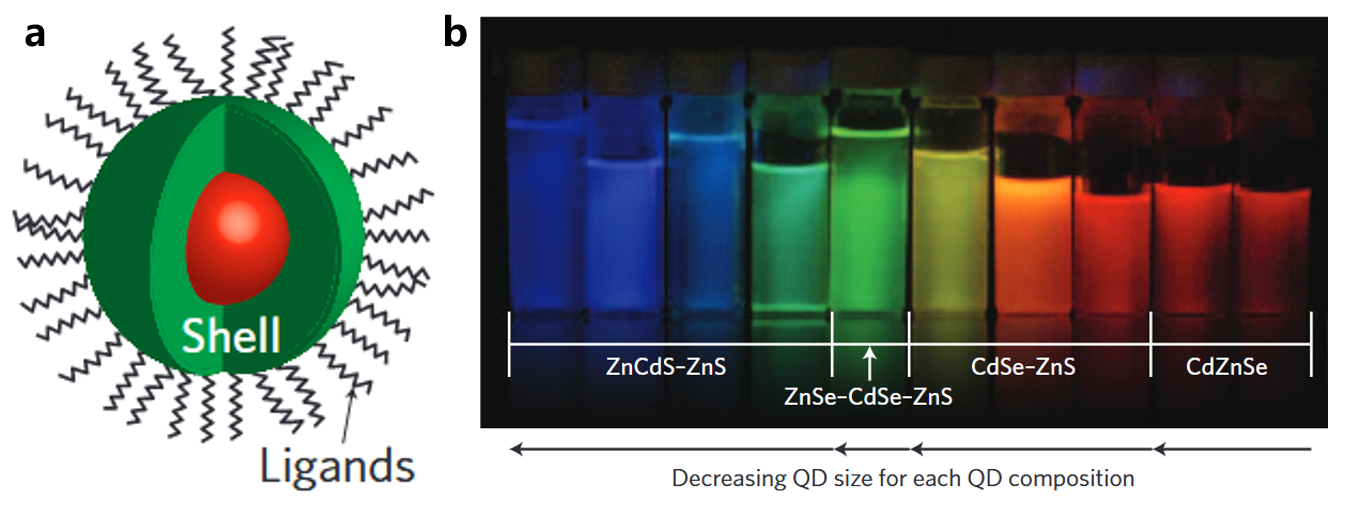
\includegraphics[width=\textwidth]{QD.png}
	\caption{胶体量子点的核壳结构和可调谐且纯净的光发射\cite{shirasaki2013emergence}。}
	\label{fig:QD}
\end{figure}
\subsection{胶体量子点发光二极管}
胶体量子点发光二极管是运用
胶体量子点光电特性自发光的技术,在外加电压下从两极注入的电子(LUMO能级)和空穴(HOMO能级)在量子点中结合形成激子,通过辐射复合发出光子。如图\ref{fig:rolloff}所示,其结构通常为阳极(Anode)/空穴注入层(Hole Injection Layer, HIL)/空穴传输层(Hole Transport Layer,HTL)/量子点发光层(Quantum Dot Emissive Layer, QDEL)/电子传输层(Electron Transport Layer, ETL)/电子注入层(Electron Injection Layer, EIL)/阴极(Cathode)。其中传输层的作用是提高对应载流子注入效率,且往往也能承担注入层的作用,为减少层与层界面带来的负面效果,我们能看到有些器件不存在注入层结构。

胶体量子点发光二极管的诞生可以分为三个阶段,最早可以追溯到1981年Alexei I. Ekimov发现了CuCl纳米晶体的量子化效应\cite{ekimov1985quantum},而在1983年Louis E. Brus率先建立了胶体量子点的理论模型\cite{brus1984electron},1994年VL Colvin等人将量子点应用到LED中,标志着QD-LED的诞生\cite{colvin1994light}。经过研究人员几十年来的不断改进创新,目前红绿蓝三色QD-LED的光致发光量子效率(Photoluminescence Quantum Efficiency, PLQY)均可做到接近100\%,而外量子效率峰值则分别达到了35\%\cite{xu2024dipole}、28.7\%\cite{deng2022solution} 和26.68\%\cite{bian2024efficient},在100cd/m$^2$初始亮度下的T$_{50}$寿命(亮度降到初值50\%的时间)分别为125,000,000 h\cite{lee2022bright}、2,570,000 h\cite{deng2022solution}、80,377 h\cite{chen2023blue}。
\begin{figure}[ht]
	\centering
	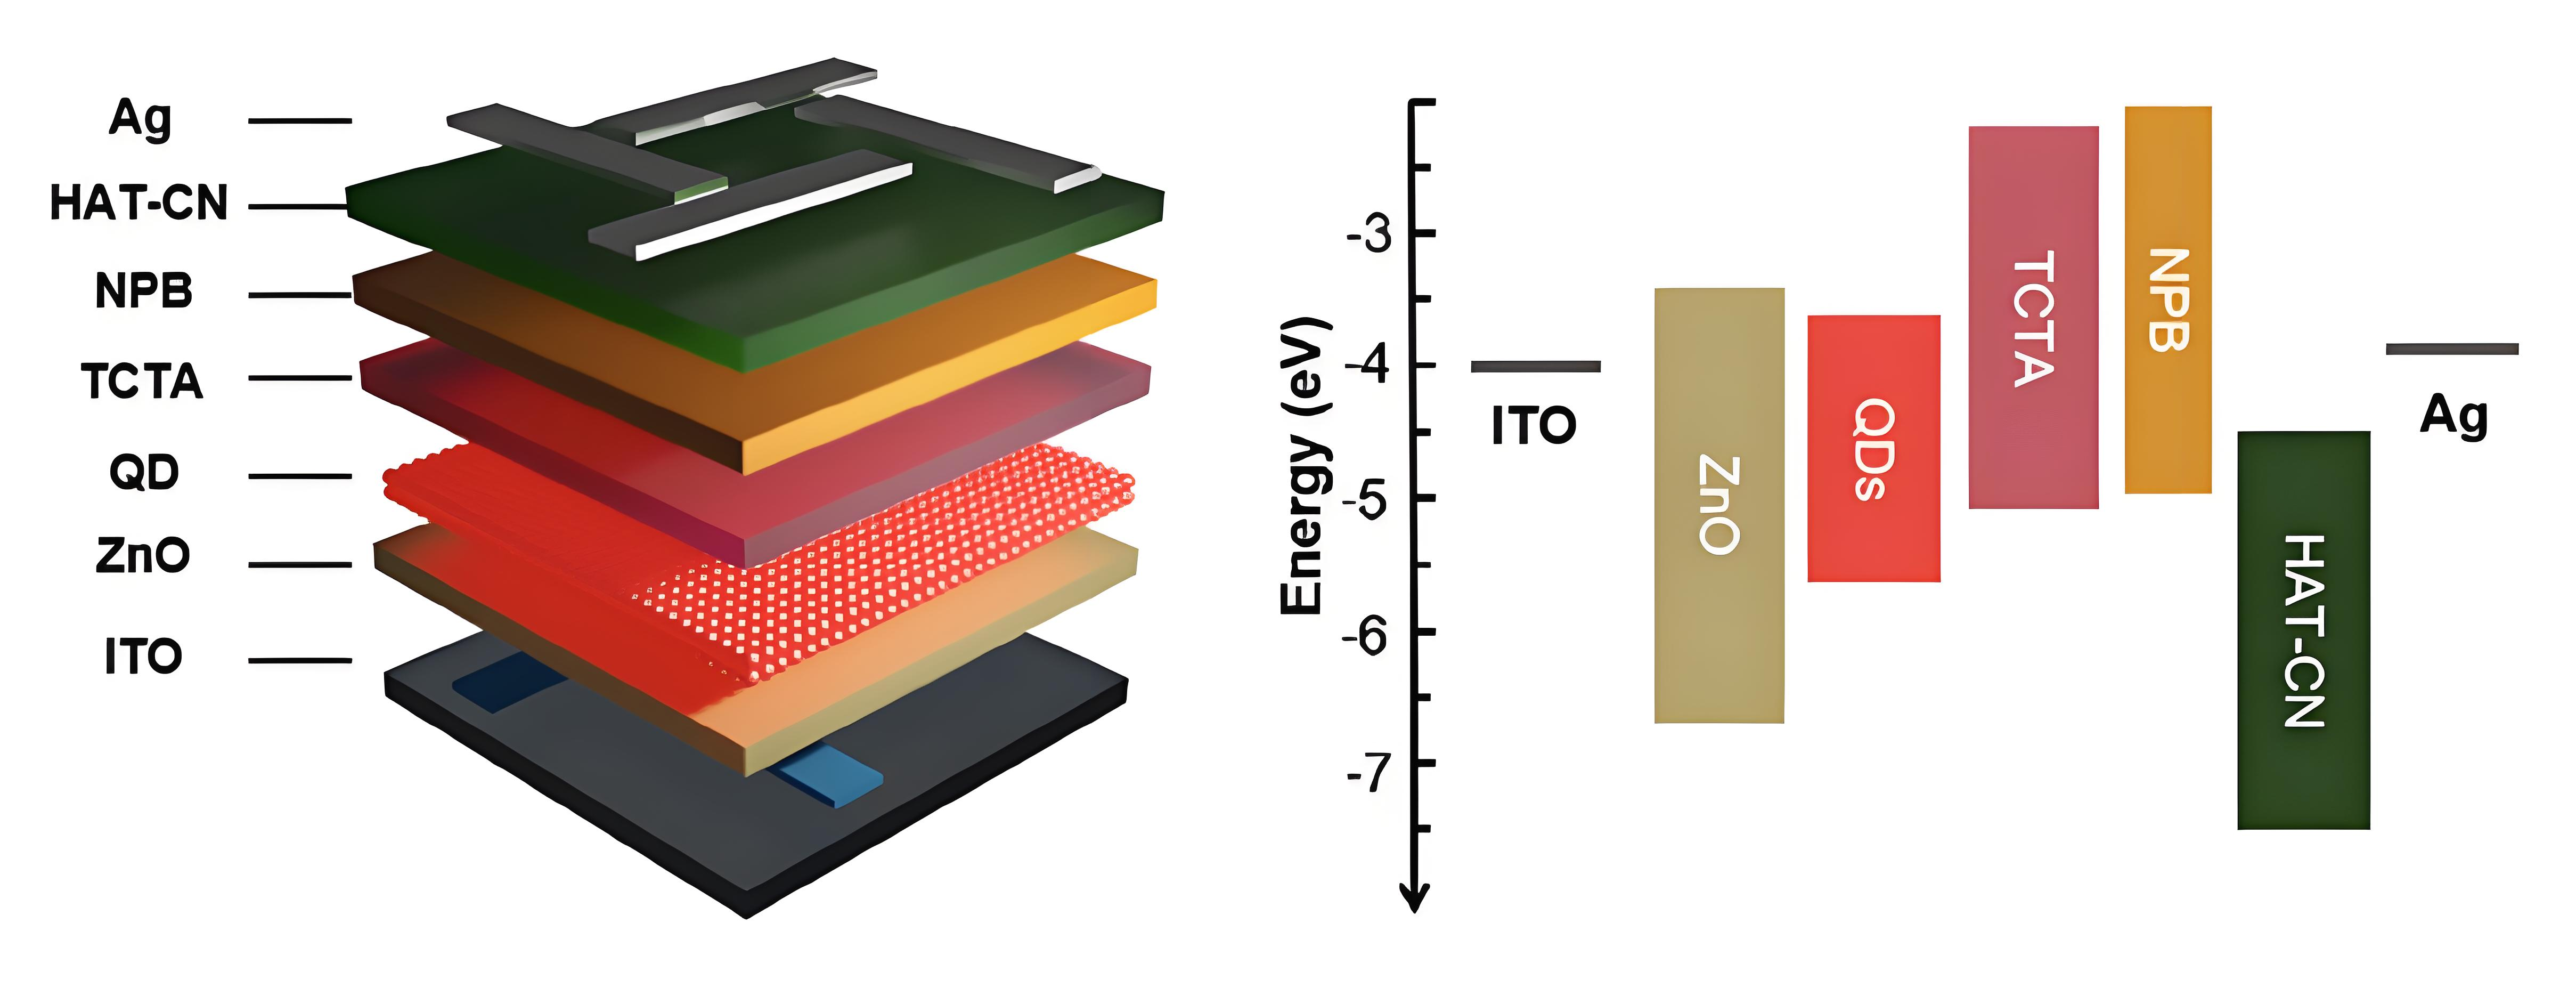
\includegraphics[width=\textwidth]{rolloff.jpeg}
	\caption{常见 QD-LED 结构与能级示意图\cite{jing2022highly}。}
	\label{fig:rolloff}
\end{figure}
\subsubsection{电致发光原理}
量子点发光二极管(QD-LED)存在光致发光(Photoluminescence, PL)与电致发光(Electroluminescence, EL)。光致发光过程:外界光子(如激光或紫外光)被量子点吸收,电子从价带跃迁至导带,形成激子(电子-空穴对),激子通过辐射复合释放光子,能量由量子点能带间隙(尺寸调控)决定,发射光谱窄(FWHM<30 nm);电致发光过程:电子和空穴分别从电子传输层(ETL,如ZnO)和空穴传输层(HTL,如TFB)注入量子点层,进一步被量子点较高的激子束缚能(>100meV)约束,电子-空穴对在量子点内部或界面处辐射复合发射光子。这里辐射复合的定义:在电子和空穴复合时,释放的能量直接转化为电磁辐射(光子);反之,能量以非光子形式(如热能、晶格振动或缺陷态跃迁)释放,即不产生光而是能量损耗,则称为非辐射复合。
\begin{figure}[ht]
	\centering
	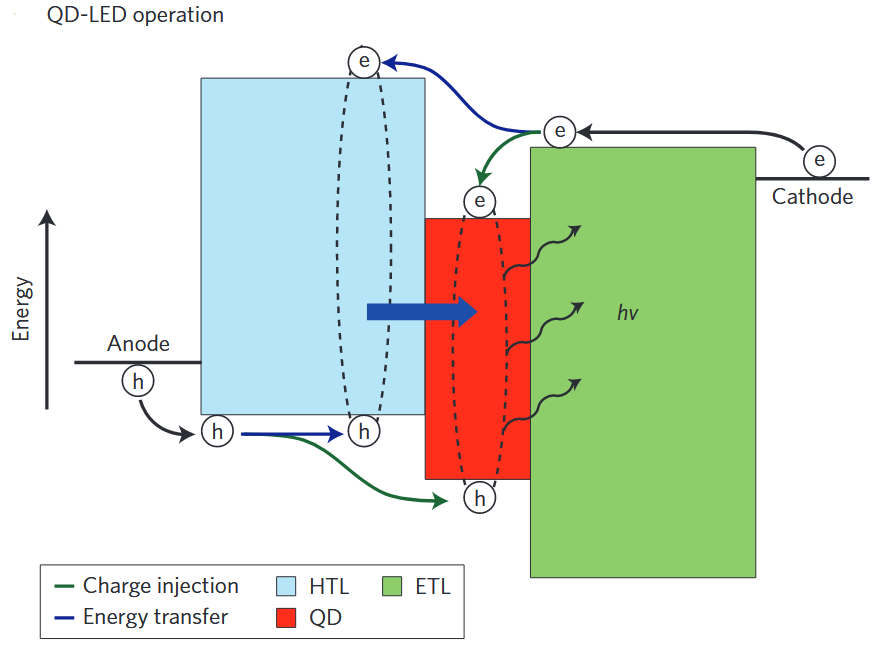
\includegraphics[width=.8\textwidth]{Snipaste.png}
	\caption{电激发原理图\cite{shirasaki2013emergence}:能量转移和直接电子注入。}
	\label{fig:EL}
\end{figure}

近年来,研究人员发现,电致发光过程除了上述QD-LED中直接电子注入形成激子外,还存在通过能量转移发光的方式,如图\ref{fig:EL}所示,由于量子点发光层较薄,电子(空穴)将穿过量子点层到达空穴(电子)传输层并与其中的空穴(电子)结合形成激子,再通过 Förster 能量共振转移(Energy Transfer, ET)机制将能量转移回量子点发光。

\subsubsection{老化机制}
老化机制通常可分为正向老化和负向老化。正向老化指的是QD-LEDs在正向偏置下的效率随时间自发提高。这种现象通常在封装后最初数十小时内最为明显。研究表明,效率提升可能源于ZnMgO或ZnO电子传输层中缺陷的钝化,这一过程通过抑制空穴漏电流来增强电子注入。Chen等人通过优化封装,QD-LEDs的外部量子效率(EQE)可达20.19\%,半衰期寿命为1,267小时,初始亮度为2,800 cd/m$^2$,分别比未优化时提高1.4倍和6.0倍\cite{Chen}。这种效率提升可能与界面反应的改善有关,铝阴极与ZnMgO层之间的反应形成AlO$_x$层,降低电子注入障碍,从而提高导电性。还有研究指出,正向老化的起源可能涉及激子猝灭机制的改变。Su等人探讨了正向老化的起源,强调界面反应的作用,如氧空位的产生增强了ZnMgO的导电性。然而,这种现象在进一步使用干燥剂封装后可能消失,表明封装条件对正向老化的影响至关重要\cite{201800549}。

而负向老化指QD-LEDs在反向偏置下的性能退化,表现为发光强度和效率的下降。研究表明,反向偏置下的大电场会显著改变载流子动力学,导致发光猝灭。机制包括量子限制斯塔克效应(QCSE)和场诱导激子解离。在高电压下,由于功能层(包括量子点层、载流子传输层、载流子注入层以及电极)的退化,器件性能持续地下降。在器件退化过程中,这些功能层会发生物理和化学反应,这些反应可能由内在因素(如界面分离、电化学反应、光化学反应以及焦耳热)和外在因素(如水和氧气的渗透及制备过程中引入的灰尘和杂质)引起。

\section{本文选题依据及主要研究内容}
目前QD-LED商业化所遇到的最大阻碍主要是器件的老化问题,无论是正向老化还是负向老化对于器件的稳定性都是一个巨大的打击。目前较多的研究结果表面,老化现象可能来源于QD-LED器件中的ZnO电子传输层。而现阶段对于QD-LED中氧化锌电子传输层的认识并不清晰,虽然研究人员已经做了大量尝试,也取得了许多突破性的结果,如双层结构、配体工程、金属离子掺杂、卤素元素掺杂等等,但这些无疑花费了大量的时间和精力,在迫切需要解决商业化问题的当下,如何得到快捷有效的方案显得尤为重要。最直截了当的方式自然是从物理底层出发,这就要求新的探测手段,以实现对器件的机理研究,从根本上给出合适的改进方案。Fan课题组率先开发出了基于电激发-光探测原理的电激发瞬态吸收(Electrically Excited Transient Absorption, EETA)光谱仪,实现了对器件中电注入载流子和电场行为的原位直接研究\cite{li2024transient,1025004826.nh}。我们知道,ZnO在室温下的带隙约3.3eV,转化为波长约为375.7nm,而目前主流的QD-LED器件的电子传输层多为ZnMgO,掺Mg后其对应波长将进一步减小,这就要求我们在375nm及更小波长范围内对QD-LED器件进行信号测量。本文基于电激发瞬态吸收光谱技术开发出了紫外波段拓展的电激发瞬态吸收光谱仪,开展对ZnO类QD-LED器件的研究。具体地,文章主要分为以下几个部分:

第一章:绪论。本章节简单介绍了QD-LED结构、机制和发展历程,以及目前商业化所遇到的问题。

第二章:电激发瞬态吸收光谱仪的原理及搭建工作(包含LabVIEW操控系统)。本章节具体介绍了电激发瞬态吸收光谱技术,基于该技术搭建了紫外波段拓展的电激发瞬态吸收光谱仪,并展示通过LaVIEW对整套仪器的一体化控制。
	
第三章:QD-LED中氧化锌类电子传输层研究。该章节主要介绍了我们基于所搭建仪器对氧化锌类电子传输层的QD-LED在紫外波段的信号研究,归属出属于ZnO的信号,展示它们在不同工作环境下的变化趋势,并给出我们的分析。

第四章:总结和展望,总结了全文的主要内容,并基于我们得到的ZnO类电子传输层结论分析未来胶体量子点发光二极管的改善方向。
